\PassOptionsToPackage{unicode}{hyperref}
\PassOptionsToPackage{naturalnames}{hyperref}

\documentclass[12pt,aspectratio=1610]{beamer}
\usecolortheme{wolverine}
\usepackage{natbib, hyperref, graphicx, amsmath}
\usepackage{xmpmulti}
\usepackage{animate}
\usepackage{bm}
\usepackage{caption}
\usepackage{mathtools}
% Custom physics notation and shorthands because I am tired of repeating it
% everywhere.
\newcommand{\mink}{\eta_{\mu\nu}}
\renewcommand{\dag}{\dagger}
\newcommand{\munu}{\mu\nu}
\newcommand{\Hint}{\hat{H}_{\text{int}}}
\newcommand{\Hab}{\hat{H}_{AB}}
\newcommand{\ahat}{\hat{a}}
\newcommand{\bhat}{\hat{b}}
\newcommand{\g}{\mathfrak{g}}
\newcommand{\BigO}{\mathcal{O}}

% The bra and ket notation.
\DeclarePairedDelimiter\bra{\langle}{\rvert}
\DeclarePairedDelimiter\ket{\lvert}{\rangle}
\DeclarePairedDelimiterX\braket[2]{\langle}{\rangle}{#1 \delimsize\vert #2}

% Some common matrix notations.
\DeclareMathOperator{\Tr}{Tr}
\DeclareMathOperator{\diag}{diag}

\setbeamertemplate{caption}[numbered]
\graphicspath{{./}{figures/}}
%Information to be included in the title page:
\pdfstringdefDisableCommands{%
\def\translate#1{#1}%
}
\title{A Gravitational Twist to Quantum Entanglement}
\author{Prateek Gupta} 
\institute{The University of Edinburgh}
\date{2023}

\begin{document}

\frame{\titlepage}
\begin{frame}{An Introduction to Quantum Gravity}
    \begin{itemize}
        \item <1-> Quantum Gravity is an active field of research.
        \item <2-> Physicists try to understand gravity at microscopic scales.
        \item <3-> Extremely difficult to study.
        \item <4-> Incompatibility with framework of QFT.
        \item <5-> Technical difficulties include non-renormalizability of GR.
        \item <6-> One of the conceptual difficulties is the nature of gravitational interactions.
        \item <7-> In GR, gravity is represented as a property of spacetime.
        \item <8-> QFT usually assumes a field propagating in a background spacetime.
    \end{itemize}
\end{frame}
\begin{frame}{An Introduction to Quantum Gravity}
    \begin{itemize}
        \item <1-> There are many candidate theories for quantum gravity, like string theory, loop quantum gravity, supergravity etc etc.
        \item <2-> None of them can be tested, yet.
        \item <3-> \textit{Known} problems, but could face \textit{unknown} problems.
        \item <4-> Due to lack of experiments, don't even know if gravity is a quantum entity!
        \item <5-> Several proposed experiments to probe this question, e.g. \citet{PhysRevD.98.126009, doi:10.1142/S0218271819430016, Bose_2017, Marletto_2017}
        \item <6-> \citet{Bose_2017} and \citet{Marletto_2017} focus on using Quantum Entanglement to probe the nature of gravity.
        \item <7-> In this talk, focus is on how gravity could entangle two masses, provided gravity was quantum in nature.
    \end{itemize}
\end{frame}

\begin{frame}{BMV Experiment}
\begin{itemize}
    \item <1-> In December 2017, two teams, \citet{Bose_2017} and \citet{Marletto_2017}, came up with an experiment to test the quantum nature of gravity.
    \item <2-> The core of this experiment was entanglement.
    \item <3-> Argued that if gravity can induce entanglement between two masses, it must be because gravity is a quantum entity! 
    \item <4-> Classical interactions $\neq$ Entanglement!\footnote{Assuming principle of locality.}
    \item <5-> The experiment is called the the Bose-Marletto-Vedral (BMV) experiment (nice review in \citet{Christodoulou_2020}).
\end{itemize}
\end{frame}

\begin{frame}{Quantum Entanglement}
    \begin{itemize}
        \item <1-> Particles in a state such that the quantum state of each constituent particle cannot be described independently of others.
        \item <2-> This could be due to number of reasons, like interacting with each other.
        \item <3-> Quantum interactions will induce entanglement!
        \item <4-> Erwin Schr\"odinger defined this as the characteristic trait of a quantum interaction \cite{schrodinger_1935}.
        \item <5-> Assume local interactions, not action at a distance.
        \item <6-> \citet{Bose_2022} uses a principle of quantum information theory, where local classical interactions cannot entangle particles.
    \end{itemize}
\end{frame}

\begin{frame}{LOCC and LOQC}
    \begin{itemize}
        \item <1> LOCC stands for ``Local Operations and Classical Communication".
        \item <2> ``Classical Communication" means the subsystems ``communicate" through classical means.
        \item <3> A central principle of quantum information theory is LOCC keeps any initially untangled state unentangled \citep{Bose_2017}.\footnote{This is under the assumption that the ``notion of classicity" itself is not extended. \citep{PhysRevA.72.062109, Hall_2018}}
        \item <4> If LOCC can’t entangle particles, the entanglement must occur through local operations and quantum communication.
        \item <5> ``Classicity" = Anything that is not quantum.
        \item <6> LOQC therefore is ``Local Operations and Quantum Communication''.
        \item <7> If mutual gravitational interaction between two masses entangles them, then the mediating gravitational field is necessarily quantum mechanical in nature.
    \end{itemize}
\end{frame}

\begin{frame}{Mechanism for Gravitationally Induced Entanglement}
    \begin{itemize}
        \item The Bose-Marletto-Vedral (BMV) experiment \citep{Christodoulou_2020} relies on two assumptions:
        \begin{enumerate}
            \item[1.] The interaction between two masses is mediated only by a gravitational field \citep{Bose_2017}, and
            \item[2.] Entanglement between two systems cannot be created by LOCC \citep{Bose_2017, Marletto_2017}.
        \end{enumerate}
        \item \citet{Bose_2022} further described a mechanism for gravity to entangle masses.
        \item They calculate a shift in the energy of the graviton vacuum due to the interaction.
        \item And subsequently a measure of entanglement called concurrence. \citep{PhysRevLett.78.5022, PhysRevA.64.042315}
        \item We further calculate Entanglement Entropy as another measure of entanglement for the same cases.
    \end{itemize}
\end{frame}

\begin{frame}{Induced Entanglement}
    \begin{itemize}
        \item Consider two matter systems in harmonic traps separated by a distance $d$, and initial state $\ket{\psi_i}=\ket{0}_A\ket{0}_B$.
        \item Let the harmonic traps be in a superposition.
        \item \begin{equation*}
    \hat{x}_{A}=-\frac{d}{2}+\delta\hat{x}_{A},\qquad \hat{x}_{B}=\frac{d}{2}+\delta\hat{x}_{B},
    \label{eq: Oscillator Locations}
\end{equation*}
\begin{equation*}
    \hat{H}_{\text{matter}} =  \frac{\hat{p}_A^2}{2m} + \frac{\hat{p}_B^2}{2m} + \frac{m\omega_m^2}{2}\delta\hat{x}^2_{A} + \frac{m\omega_m^2}{2}\delta\hat{x}^2_{B},
\end{equation*}
\begin{equation*} \label{eq: ModeOp1}
    \delta\hat{x}_{A} = \sqrt{\frac{\hbar}{2m\omega_m}}(\hat{a} + \hat{a}^{\dag}), \qquad \delta\hat{x}_{B} = \sqrt{\frac{\hbar}{2m\omega_m}}(\hat{b} + \hat{b}^{\dag}),
\end{equation*}
\begin{equation*} \label{eq: ModeOp2}
    \hat{p}_A = i\sqrt{\frac{\hbar m\omega_m}{2}}(\hat{a} - \hat{a}^{\dag}), \qquad \hat{p}_B = i\sqrt{\frac{\hbar m\omega_m}{2}}(\hat{b} - \hat{b}^{\dag}),
\end{equation*}
    \end{itemize}
\end{frame}
\begin{frame}{Induced Entanglement}
    \begin{itemize}
        \item Introduce a small interaction potential, $\lambda H_{AB}$, and the perturbed final state is given by, $$\ket{\psi_{\text{f}}}\equiv\frac{1}{\mathcal{\sqrt{N}}}\sum_{n,N}C_{nN}\ket{n}\ket{N},$$ where $\mathcal{N}=\sum_{n,N}\vert C_{nN}\vert^{2}$, $\ket{n}$ and $\ket{N}$ are numbered states.
        \item The coefficient of the unperturbed state is $C_{00} = 1$, and the remaining are given by \citep{Bose_2022}, $$C_{nN} =\lambda\frac{\langle n\vert\langle N\vert\hat{H}_{AB}\vert0\rangle\vert0\rangle}{2E_{0}-E_{n}-E_{N}}$$
        \item If the interaction was classical, the remaining coefficients would be $0$ due to orthogonality of $\ket{n}\ket{N}$ and $\ket{0}\ket{0}$.
    \end{itemize}
\end{frame}
\begin{frame}{Induced Entanglement}
    If we set $A_n \equiv C_{n0}$ and $B_N \equiv C_{0N}$, then we can write the perturbed state as \citep{Bala_2012, Bose_2022},
\begin{equation*}
    \begin{aligned}
        \ket{\psi_f} &= \frac{1}{\sqrt{\mathcal{N}}} \Bigg(\ket{0}\ket{0} + \sum_{n>0} A_n \ket{n}\ket{0} + \sum_{N>0} B_N \ket{0}\ket{N} + \sum_{n, N > 0} C_{nN} \ket{n}\ket{N}\Bigg) \\
        &= \frac{1}{\sqrt{\mathcal{N}}} \Bigg( \Big(\ket{0} + \sum_{n>0} A_n \ket{n}\Big)\Big(\ket{0} + \sum_{N>0} B_N \ket{N}\Big) + \sum_{n, N > 0} (C_{nN} - A_nB_N) \ket{n}\ket{N} \Bigg)\\
    \end{aligned}
\end{equation*}
\begin{itemize}
    \item The first term would yield a separable state, second an entangled state.
    \item It shows the stark difference between LOCC and LOQC.
\end{itemize}
\end{frame}

\begin{frame}{Concurrence}
    \begin{itemize}
        \item The density matrix for the system is given by $$\hat{\rho}_{A}=\sum_{N_B}\braket{N_B}{\psi_{\text{f}}}\braket{\psi_{\text{f}}}{N_B} = \frac{1}{\mathcal{N}}\sum_{n,n',N}C_{nN}C_{n'N}^{*}\ket{n}\bra{n'}$$ \citep{Bose_2022}
        \item Thus the concurrence can be calculated by $$C\equiv\sqrt{2(1-\text{tr}[\hat{\rho}_{A}^{2}])}$$ \citep{PhysRevLett.78.5022, PhysRevA.64.042315}
        \item \begin{equation*}
    C = \sqrt{2\bigg(1 - \frac{1}{\mathcal{N}^2}\sum_{n,n',N,N'}C_{nN}C^{*}_{n'N} C_{n'N'}C^{*}_{nN'}\bigg)}
    \label{eq: Concurrence}
    \end{equation*}
        \item For an unentangled system, $C = 0$, and $\sqrt{2}$ for a maximally entangled system\footnote{with an infinite dimensional Hilbert Space}.
    \end{itemize}
\end{frame}

\begin{frame}{Entanglement Entropy}
    \begin{itemize}
        \item Another measurement of the degree of entanglement is the von Neumann Entanglement Entropy \citep{Bala_2012, PhysRevA.101.052110, suddho}.
        \item \begin{equation*}
            \mathcal{S}(\hat{\rho}_A) = -\Tr(\hat{\rho}_A \log{\hat{\rho}_A})
        \end{equation*}
        \item This can be calculated relatively easily by calculating the logarithm of the density operator, which is diagonizable.
        \item We have seen that quantum interactions induce entanglement, and that Concurrence and Entanglement Entropy.
    \end{itemize}
\end{frame}

\begin{frame}{Linearization of Gravity}
    \begin{itemize}
        \item Now that we know quantum interactions induce entanglement, we want to substitute the general quantum interaction with a quantum gravitational interaction.
        \item To do that, we must first understand how gravity is quantized.
        \item And to do that, we must understand how Einstein's Field Equations can be linearized.
    \end{itemize}
\end{frame}

\begin{frame}{Linearization of Gravity}
    \begin{itemize}
        \item Follow the same procedure as \citet{Gupta_1952}, with minor modifications.
        \item Consider the Einstein Field Equations, $R^{\munu} - \frac{1}{2}Rg^{\munu} = -\frac{1}{2}\kappa^2T^{\munu}$.
        \item Covariant divergence of the Stress-Energy tensor is $0$, so we can write a Stress-Energy tensor \textit{density} $\mathfrak{T}^{\munu} = \sqrt{-g}T^{\munu}$ (where $g$ is the determinant of the metric).
        \item \begin{equation*}
    \frac{\partial\mathfrak{T}^{\nu}_{\mu}}{\partial x^{\nu}} - \frac{1}{2}\mathfrak{T}^{\alpha\beta}\frac{\partial g_{\alpha\beta}}{\partial x^{\mu}} = 0.
    \end{equation*}
    \item Define Stress-Energy \textit{pseudo-tensor density} \citep{Gupta_1952} for the gravitational field, satisfying the equation,
\begin{equation*}
    \frac{\partial t^{\nu}_{\mu}}{\partial x^{\nu}} = - \frac{1}{2}\mathfrak{T}^{\alpha\beta}\frac{\partial g_{\alpha\beta}}{\partial x^{\mu}}.
\end{equation*}
    \item Then the conservation of stress-energy tensor can be written as,
    \begin{equation*}
    \frac{\partial}{\partial x^{\nu}}(\mathfrak{T}^{\nu}_{\mu} + t^{\nu}_{\mu}) = 0
    \label{eq: PseudoStEnergyDen1}
\end{equation*}
    \end{itemize}
\end{frame}
\begin{frame}{Linearization of Gravity}
    \begin{itemize}
        \item Following \citet{Gupta_1952} and \citet{EinsteinGravWave} we can obtain a linear approximation for the field by considering small perturbations $h_{\munu}$.
        \item $$g_{\munu} = \mink + h_{\munu},$$ where $\mink = \diag(-1, +1, +1, +1)$.
        \item It is also convenient to decompose $h_{\munu}$ as $h_{\munu} = \gamma_{\munu} - \frac{1}{2}\mink\gamma,$ where $\gamma = \gamma_{\lambda\lambda}$.
        \item Choose coordinate/supplementary conditions given by \citep{Gupta_1952},
        \begin{equation*}
            \frac{\partial h_{\munu}}{\partial x_{\nu}} -  \frac{1}{2}\frac{\partial h_{\lambda\lambda}}{\partial x_{\mu}} = 0
        \end{equation*}
    \end{itemize}
\end{frame}
\begin{frame}{Linearization of Gravity}
    \begin{itemize}
        \item Thus, simplifying the Einstein equations with these constraints, we get,
        \begin{equation*}
            \frac{\partial t_{\munu}}{\partial x_{\nu}} = \frac{\kappa^2}{2}\frac{\partial \gamma_{\nu\lambda}}{\partial x_{\mu}}T_{\nu\lambda} - \frac{\kappa^2}{4}\frac{\partial \gamma}{\partial x_{\mu}}T_{\nu\nu}
        \end{equation*}
        \begin{equation*}
            \frac{\partial \gamma_{\munu}}{\partial x_{\nu}} = 0
        \end{equation*}
        \begin{equation*}
            \Box^2\gamma_{\munu} = \kappa^2T_{\munu}
        \end{equation*}
        \item These are only valid in a first order approximation.
        \item One can now find the Hamiltonian density by solving for $t_{\munu}$ and calculating $t_{00}$.
        \item \begin{equation*}
    H = t_{00} = \frac{1}{2}\Bigg[\frac{\partial\gamma_{\lambda\rho}}{\partial t}\frac{\partial\gamma_{\lambda\rho}}{\partial t} - \frac{1}{2}\frac{\partial\gamma}{\partial t}\frac{\partial\gamma_{\rho\rho}}{\partial t} + \frac{1}{2}\Bigg(\frac{\partial\gamma_{\lambda\rho}}{\partial x_{\sigma}}\frac{\partial\gamma_{\lambda\rho}}{\partial x_{\sigma}} - \frac{1}{2}\frac{\partial\gamma}{\partial x_{\sigma}}\frac{\partial\gamma_{\rho\rho}}{\partial x_{\sigma}}\Bigg)\Bigg]
\end{equation*}
    \end{itemize}
\end{frame}

\begin{frame}{Canonical Quantization}
    \begin{itemize}
        \item Now that we have the Hamiltonian, we can proceed to do a canonical quantization, again following \citet{Gupta_1952}.
        \item The Lagrangian Density is given by,
        \begin{equation*}
    L = -\frac{1}{4}\Bigg(\frac{\partial\gamma_{\munu}}{\partial x_{\lambda}}\frac{\partial\gamma_{\munu}}{\partial x_{\lambda}} - \frac{1}{2}\frac{\partial\gamma}{\partial x_{\lambda}}\frac{\partial\gamma}{\partial x_{\lambda}}\Bigg)
\end{equation*}
        \item We can calculate the canonical conjugate of $\gamma_{\munu}$ and $\gamma$ using,
        \begin{equation*}
    \pi_{\munu} = \frac{\partial L}{\partial (\partial \gamma_{\munu}/\partial t)} = \frac{1}{2}\frac{\partial \gamma_{\munu}}{\partial t}
\end{equation*}
\begin{equation*}
    \pi = \frac{\partial L}{\partial (\partial \gamma/\partial t)} = -\frac{1}{4}\frac{\partial \gamma}{\partial t}
\end{equation*}
    \end{itemize}
\end{frame}

\begin{frame}{Canonical Quantization}
    \begin{itemize}
        \item The ETCRs are found to be,
        \begin{equation*}
            [\gamma_{\munu}(x), \pi_{\lambda\rho}(x')] = i(\eta_{\mu\lambda}\eta_{\nu\rho} + \eta_{\mu\rho}\eta_{\nu\lambda})\delta(\bm{x}-\bm{x'}),
        \end{equation*}
        \begin{equation*}
            [\gamma(x), \pi(x')] = -4i\delta(\bm{x}-\bm{x'}).
        \end{equation*}
        \item The perturbations can be written in an operator valued form \citep{Bose_2022}, $$\hat{h}_{\mu\nu}=\mathcal{A}\int d\bm{k}\sqrt{\frac{\hbar}{2\omega_{\bm{k}}(2\pi)^{3}}}(\hat{P}_{\mu\nu}^{\dagger}(\bm{k)}e^{-i\bm{k}\cdot\bm{r}}+\text{h.c}),$$
        where ${\bm{k}}$ is the three-vector, $d{\bm{k}}\equiv d^{3}k$. 
        \item $\hat{P}_{\mu\nu}$ \& $\hat{P}_{\mu\nu}^{\dagger}$ are the graviton annihilation and the creation operators, and $\mathcal{A}=\sqrt{16\pi G/c^{2}}$.
    \end{itemize}
\end{frame}
\begin{frame}{Canonical Quantization}
    \begin{itemize}
        \item Thus we get an on-shell spin-2 graviton through $\gamma_{\munu}$ and an off-shell spin-0 graviton through $\gamma$ given by,
        \begin{equation*}
    \hat{\gamma}_{\munu} = \mathcal{A}\int d\bm{k} \sqrt{\frac{\hbar}{2\omega_k(2\pi)^3}}(\hat{P}_{\munu}^{\dagger}(\bm{k})e^{-i\bm{k}\cdot\bm{r}} + \hat{P}_{\munu}(\bm{k})e^{i\bm{k}\cdot\bm{r}}),
\end{equation*}
\begin{equation*}
    \hat{\gamma} = 2\mathcal{A}\int d\bm{k} \sqrt{\frac{\hbar}{2\omega_k(2\pi)^3}}(\hat{P}^{\dagger}(\bm{k})e^{-i\bm{k}\cdot\bm{r}} + \hat{P}(\bm{k})e^{i\bm{k}\cdot\bm{r}}).
\end{equation*}
\item The ETCRs for the mode operators are,
\begin{equation*}
    [\hat{P}_{\munu}(\bm{k}), \hat{P}_{\lambda\rho}^{\dagger}(\bm{k'})] = (\eta_{\mu\lambda}\eta_{\nu\rho} + \eta_{\mu\rho}\eta_{\nu\lambda})\delta(\bm{k} - \bm{k'}),
\end{equation*}
\begin{equation*}
    [\hat{P}(\bm{k}), \hat{P}^{\dagger}(\bm{k'})] = -\delta(\bm{k} - \bm{k'}).
\end{equation*}
\item Finally, the graviton vacuum energy is given by,
\begin{equation*}
    \hat{H}_g = \int d\bm{k}\,\hbar\omega_k\bigg(\frac{1}{2}\hat{P}_{\munu}^{\dagger}(\bm{k})\hat{P}^{\munu}(\bm{k}) - \hat{P}^{\dagger}(\bm{k})\hat{P}(\bm{k})\bigg).
\end{equation*}
    \end{itemize}
\end{frame}

\begin{frame}{Quantum Gravitational Interaction}
    \begin{itemize}
        \item $$\hat{H}_{\text{int}}=-\frac{1}{2}\int d\bm{r}\hat{h}^{\mu\nu}(\bm{r})\hat{T}_{\mu\nu}(\bm{r})$$
        \item The first order contribution to the shift in energy is zero, i.e. $\bra{0}\Hint\ket{0} = 0$.
        \item Thus the shift in the graviton vacuum energy is given by the second order perturbation theory,
        \begin{equation*}
    \Delta \hat{H}_{g} \equiv \sum \int d\bm{k} \,\frac{\bra{0}\Hint\ket{\bm{k}}\bra{\bm{k}}\Hint\ket{0}}{E_0 - E_{\bm{k}}}.
\end{equation*}
\item The sum indicates summation over all one particle projectors $\ket{\bm{k}}\bra{\bm{k}}$, and $E_{\bm{k}} = E_0 + \hbar\omega_k$.
\item This defines the quantum gravitational interaction and now we can find the induced entanglement.
    \end{itemize}
\end{frame}

\begin{frame}{Entanglement in Static Limit}
\begin{itemize}
    \item In this case, stress energy tensor is $$\hat{T}_{00}(\bm{r})\equiv mc^{2}(\delta(\bm{r}-\hat{\bm{r}}_{A})+\delta(\bm{r}-\hat{\bm{r}}_{B}))$$ \citep{Bose_2022}. This is the non-relativistic limit.
    \item \begin{equation*}
    \begin{aligned}
        \Hint &= -\frac{1}{2} \int d{\bm{r}} \mathcal{A}\int d\bm{k'} \sqrt{\frac{\hbar}{2\omega_{k'} (2\pi)^3}}\Big(\hat{P}_{00}^{\dagger}(\bm{k'})e^{-i\bm{k'}\cdot\bm{r}}\\
        &\qquad\qquad\qquad+ \hat{P}^{\dagger}(\bm{k'})e^{-i\bm{k'}\cdot\bm{r}} + \text{H.c.} \Big)\hat{T}_{00}(\bm{r})
    \end{aligned}
    \end{equation*}
    \item The shift in the graviton vacuum energy in this case is then given by, $$\Delta{\hat{H}_{g}}\equiv\int d\bm{k}\frac{\langle0\vert\hat{H}_{\text{int}}\vert\bm{k}\rangle\langle\bm{k}\vert\hat{H}_{\text{int}}\vert0\rangle}{E_{0}-E_{\bm{k}}}$$
    \item  $\ket{k} = (\hat{P}_{00}^{\dagger}(\bm{k}) + \hat{P}^{\dagger}(\bm{k})) \ket{0}$ is the one particle state constructed in the unperturbed background, $E_{\bm{k}} = E_0 + \hbar\omega_k$
\end{itemize}
\end{frame}

\begin{frame}{Entanglement in Static Limit}
\begin{itemize}
    \item Thus, we get, \begin{equation*}
    \Delta \hat{H}_g = -\frac{Gm^2}{|\hat{x}_a - \hat{x}_b|}.
\end{equation*}
    \item This is the Newtonian potential!
    \item The lowest order interaction term is $\Hab = \frac{2Gm^{2}}{d^{3}}\,\delta\hat{x}_{A}\delta\hat{x}_{B}$
    \item The final state is given by,
    \begin{equation*}
    \vert\psi_{f}\rangle\equiv\frac{1}{\sqrt{1+(\mathfrak{g}/(2\omega_{m}))^{2}}}[\vert0\rangle\vert0\rangle-\frac{\mathfrak{g}}{2\omega_{m}}\vert1\rangle\vert1\rangle].
\end{equation*}
\item Where we define the coupling, $\mathfrak{g}$, as, $\mathfrak{g} = \frac{Gm}{d^3\omega_m}.$
    \item Thus, the concurrence is given by, $$C=\frac{Gm}{d^3\omega_m^2}$$
\end{itemize}
\end{frame}

\begin{frame}{Entanglement in Non-Static Case}
\begin{itemize}
    \item In this case, stress energy tensor once again given by the interaction Hamiltonian, but is more complicated since the system is no longer static.
    \item Specifically, we consider two particles in QHOs moving along the $x$-axis such that the only non-zero components of $T_{\munu}$ are given by $T_{00}$, $T_{01} = T_{10}$, and $T_{11}$. 
    \item Following the exact same method as in the previous case, we get that the shift in the graviton vacuum energy in this case is then given by, $$\Delta\hat{H}_{g} =-\frac{Gm^{2}}{\vert{\hat{x}}_{A}-{\hat{x}}_{B}\vert} -\frac{G(3{\hat{p}}_{A}^{2}-8\hat{p}_{A}\hat{p}_{B}+3{\hat{p}}_{B}^{2})}{2c^{2}\vert{\hat{x}}_{A}-{\hat{x}}_{B}\vert} -\frac{G(5{\hat{p}}_{A}^{4}-18{\hat{p}}_{A}^{2}{\hat{p}}_{B}^{2}+5{\hat{p}}_{B}^{4})}{8c^{4}m^{2}\vert{\hat{x}}_{A}-{\hat{x}}_{B}\vert}$$
    \item There are now relativistic corrections to the Newtonian potential.
    \item Let us term them ``Correction-1'' and ``Correction-2''.
\end{itemize}
\end{frame}

\begin{frame}{Correction-1}
    \begin{itemize}
        \item The lowest order interaction term in this correction is given by,
        \begin{equation*}
    \Hab  \approx \frac{4G\hat{p}_{A}\hat{p}_{B}}{c^{2}d} + \ldots
\end{equation*}
\item The final state can now be calculated to be,
\begin{equation*}
    \vert\psi_{f}\rangle\equiv\frac{1}{\sqrt{1+(\mathfrak{g}/(2\omega_{m}))^{2}}}[\vert0\rangle\vert0\rangle+\frac{\mathfrak{g}}{2\omega_{m}}\vert1\rangle\vert1\rangle].
\end{equation*}
\item Where the coupling is, $\g = \frac{2Gm\omega_m}{c^2d}$.
\item The concurrence for this correction then is  $$C = \frac{2Gm}{c^2d}.$$
    \end{itemize}
\end{frame}

\begin{frame}{Correction-2}
    \begin{itemize}
        \item The lowest order interaction term in this correction is given by,
        \begin{equation*}
    \Hab \approx \frac{9G{\hat{p}}_{A}^{2}{\hat{p}}_{B}^{2}}{4c^{4}m^{2}d} + \ldots
\end{equation*}
\item The final state can now be calculated to be,
\begin{equation*}
     \vert\psi_{f}\rangle\equiv\frac{1}{\sqrt{1+(\mathfrak{g}/(2\omega_{m}))^{2}}}[\vert0\rangle\vert0\rangle-\frac{\mathfrak{g}}{2\omega_{m}}\vert2\rangle\vert2\rangle].
\end{equation*}
\item Where the coupling is, $\g = \frac{9G\hbar\omega_m^2}{16c^4d}$.
\item The concurrence for this correction then is  $$C = \frac{9G\hbar\omega_m}{16c^4d}.$$
    \end{itemize}
\end{frame}

\begin{frame}{Calculation of Entanglement Entropy}
    \begin{itemize}
        \item Each of the previous cases has similar final state and a common expression for the density matrix as a function of the coupling.
        \item If we were to define $\xi = \frac{\g}{2\omega_m}$, then the density matrix for each case is given by,
        \begin{equation*}
    \rho_A(\xi(\mathfrak{g})) = \frac{1}{1+\xi^2}\begin{bmatrix}
        1 && 0\\
        0 && \xi^2
    \end{bmatrix},
\end{equation*}
    \item Common expression for the entanglement entropy,
    $$\mathcal{S}(\rho_A(\mathfrak{g})) = \log\Bigg(1+ \Big(\frac{\mathfrak{g}}{2\omega_{m}}\Big)^2\Bigg) - \frac{2\Big(\frac{\mathfrak{g}}{2\omega_{m}}\Big)^2}{1+\Big(\frac{\mathfrak{g}}{2\omega_{m}}\Big)^2}\log\Big(\frac{\mathfrak{g}}{2\omega_{m}}\Big).$$
    \item We can further approximate this to be,
    \begin{equation*}
    \mathcal{S}_A \approx {\xi}^2 \Big((1 - 2\log(\xi)\Big) + \xi^4 \Big(2\log(\xi) - \frac{1}{2}\Big) + \mathcal{O}(\xi^6),
\end{equation*}
    \end{itemize}
\end{frame}

\begin{frame}{Calculation of Entanglement Entropy}
    \begin{itemize}
        \item Thus we can now simply plug in the coupling for each case, and get the entanglement entropy.
        \item Static case:
        \begin{equation*}
    \mathcal{S}_A \approx \Big({\frac{Gm}{2d^3\omega_m^2}}\Big)^2 \Big((1 - 2\log\Big({\frac{Gm}{2d^3\omega_m^2}}\Big)\Big) + \Big({\frac{Gm}{2d^3\omega_m^2}}\Big)^4 \Big(2\log\Big({\frac{Gm}{2d^3\omega_m^2}}\Big) - \frac{1}{2}\Big)
\end{equation*}
\item Non-static Correction-1:
$$\mathcal{S}_A \approx \Big(\frac{Gm}{c^2d}\Big)^2 \Big((1 - 2\log\Big(\frac{Gm}{c^2d}\Big)\Big) + \Big(\frac{Gm}{c^2d}\Big)^4 \Big(2\log\Big(\frac{Gm}{c^2d}\Big) - \frac{1}{2}\Big)$$
\item Non-Static Correction-2:
$$\mathcal{S}_A \approx \Big(\frac{9G\hbar\omega_m}{32c^4d}\Big)^2 \Big((1 - 2\log\Big(\frac{9G\hbar\omega_m}{32c^4d}\Big)\Big) + \Big(\frac{9G\hbar\omega_m}{32c^4d}\Big)^4 \Big(2\log\Big(\frac{9G\hbar\omega_m}{32c^4d}\Big) - \frac{1}{2}\Big).$$
    \end{itemize}
\end{frame}

\begin{frame}{Comparisons}
    \begin{itemize}
        \item Both Concurrence and Entanglement Entropy have non-zero positive values for each case.
        \item Expressions for Coupling, Concurrence and Entanglement Entropy easier to understand with a visualisation.
        \item Take mass as $10^{-14}$ Kg, and $\omega_m = 10^8$ Hz as fixed. Then we can plot the quantities against distance.
    \end{itemize}
\end{frame}

\begin{frame}{Comparisons}
    \begin{figure}
            \centering
            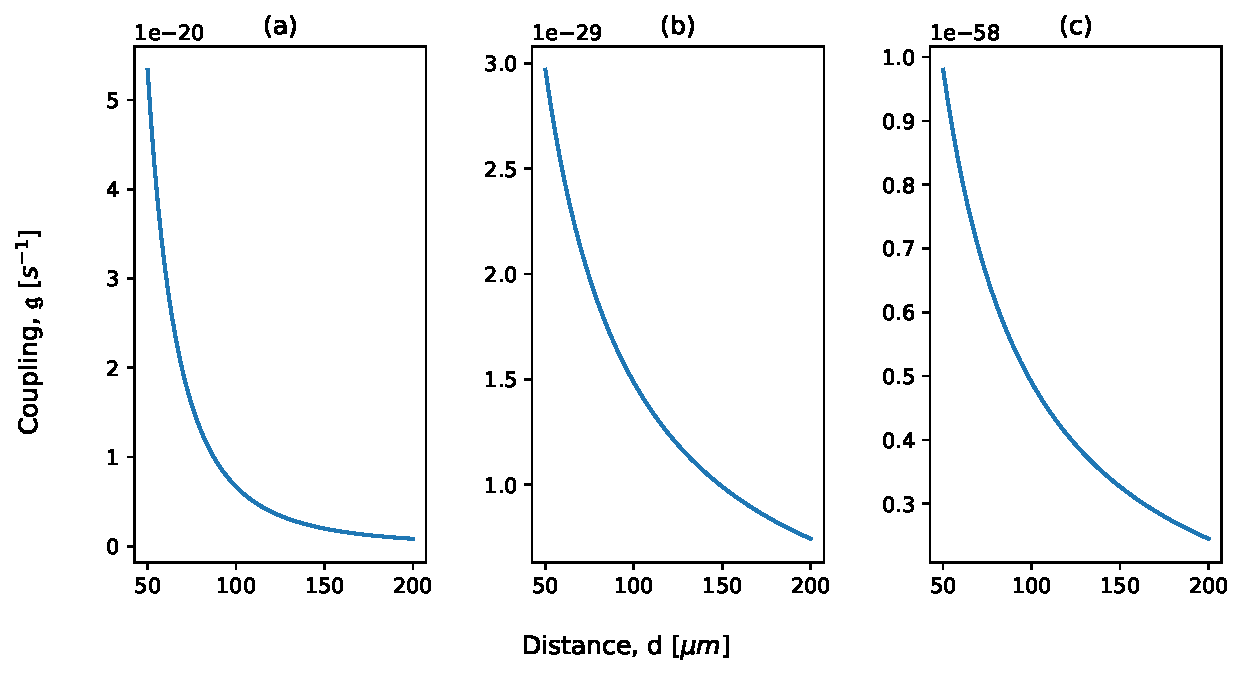
\includegraphics[width=12cm]{Coupling.pdf}
            \captionsetup{labelformat=empty}
            \caption{\footnotesize{Comparison of Coupling for Different Cases:  (a) Static Case; (b) Non-static Correction $1$ (c) Non Static Correction $2$}}
            \label{fig:Coupling}
        \end{figure}
\end{frame}

\begin{frame}{Comparisons}
    \begin{figure}
            \centering
            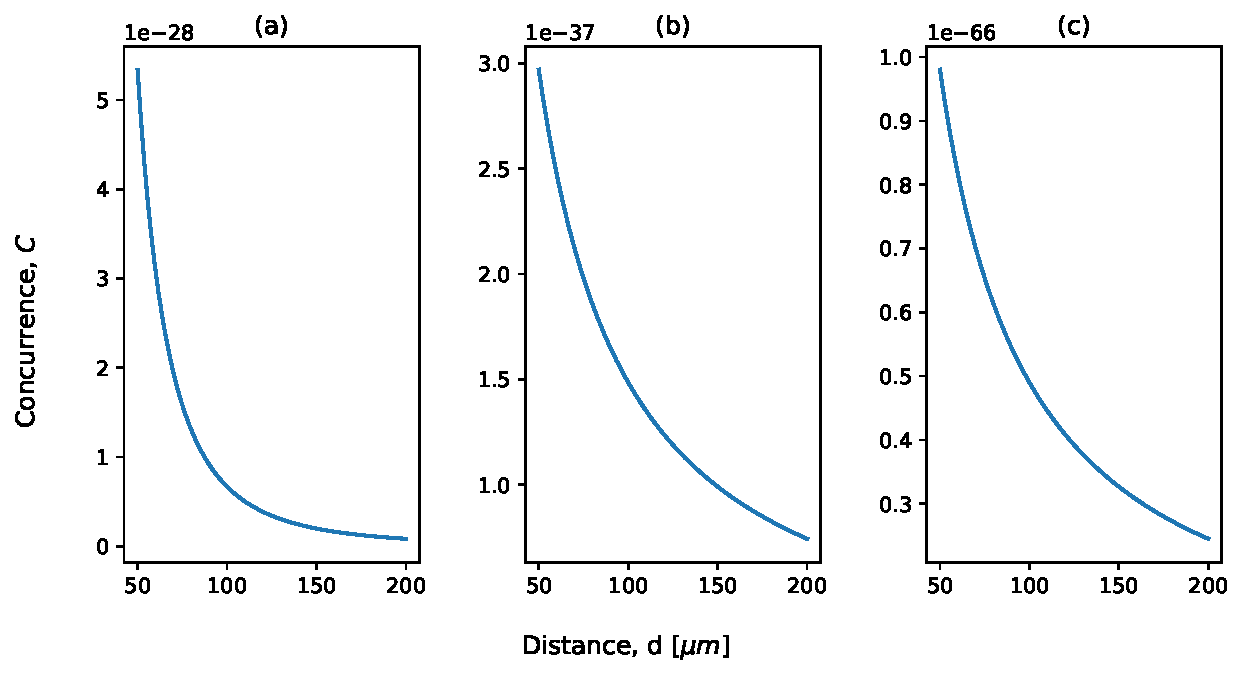
\includegraphics[width=12cm]{ConcCases.pdf}
            \captionsetup{labelformat=empty}
            \caption{\footnotesize{Comparison of Concurrence for Different Cases:  (a) Static Case; (b) Non-static Correction $1$ (c) Non Static Correction $2$}}
            \label{fig:ConcCases}
        \end{figure}
\end{frame}

\begin{frame}{Comparisons}
    \begin{figure}
            \centering
            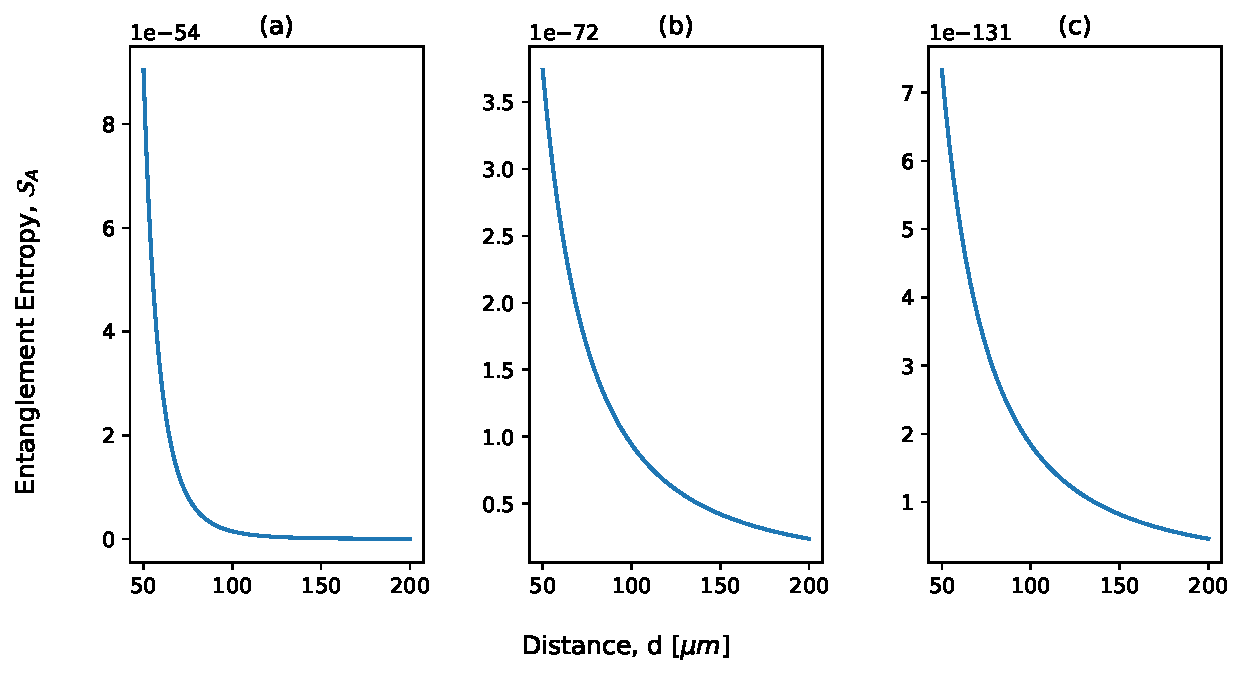
\includegraphics[width=12cm]{EECases.pdf}
            \captionsetup{labelformat=empty}
            \caption{\footnotesize{Comparison of Entanglement Entropy for Different Cases:  (a) Static Case; (b) Non-static Correction $1$ (c) Non Static Correction $2$}}
            \label{fig:EE}
        \end{figure}
\end{frame}

\begin{frame}{Summary}
\begin{itemize}
    \item We have talked about the recent table-top experiments to probe the quantum nature of gravity.
    \item We then talked about how Entanglement can be used to determine if gravity is a quantum entity.
    \item Next, we explored how entanglement is induced by quantum interactions.
    \item Then, in order to use a quantum gravitational interaction, we saw how gravity can be linearized and then quantized.
    \item We then calculated the shift in the graviton vacuum energy for an interaction between two particles in different cases, static and non-static.
    \item We finally calculated the two measures of entanglement, Concurrence and Entanglement Entropy.
    \item For each case, they yielded non-zero positive values. Thus, if gravity is a quantum entity, we can detect entanglement between two particles.
\end{itemize}    
\end{frame}

\begin{frame}{Conclusion}
\begin{itemize}
    \item Quantum entanglement can be used to confirm that gravity indeed is a quantum entity!
    \item This can be verified using table-top experiments.
    \item If classical interactions cannot entangle masses, and gravity does entangle masses, then gravity must be quantum natured. \citep{Bose_2017, Marletto_2017}
    \item This study was mainly done using a flat background spacetime. It will be interesting to see the results of these calculations done on a curved spacetime.
    \item Results on deSitter spacetime particularly interesting due to cosmological reasons.
\end{itemize}
    
\end{frame}


\begin{frame}[allowframebreaks]{References}

\bibliography{sources}
\bibliographystyle{aasjournal}

\end{frame}

\end{document} 